\documentclass{beamer}
\mode<presentation>
\usepackage{amsmath}
\usepackage{amssymb}
%\usepackage{advdate}
\usepackage{adjustbox}
\usepackage{subcaption}
\usepackage{enumitem}
\usepackage{multicol}
\usepackage{listings}
\usepackage{url}
\def\UrlBreaks{\do\/\do-}
\usetheme{Boadilla}
\usecolortheme{lily}
\setbeamertemplate{footline}
{
  \leavevmode%
  \hbox{%
  \begin{beamercolorbox}[wd=\paperwidth,ht=2.25ex,dp=1ex,right]{author in head/foot}%
    \insertframenumber{} / \inserttotalframenumber\hspace*{2ex} 
  \end{beamercolorbox}}%
  \vskip0pt%
}
\setbeamertemplate{navigation symbols}{}

\providecommand{\nCr}[2]{\,^{#1}C_{#2}} % nCr
\providecommand{\nPr}[2]{\,^{#1}P_{#2}} % nPr
\providecommand{\mbf}{\mathbf}
\providecommand{\pr}[1]{\ensuremath{\Pr\left(#1\right)}}
\providecommand{\qfunc}[1]{\ensuremath{Q\left(#1\right)}}
\providecommand{\sbrak}[1]{\ensuremath{{}\left[#1\right]}}
\providecommand{\lsbrak}[1]{\ensuremath{{}\left[#1\right.}}
\providecommand{\rsbrak}[1]{\ensuremath{{}\left.#1\right]}}
\providecommand{\brak}[1]{\ensuremath{\left(#1\right)}}
\providecommand{\lbrak}[1]{\ensuremath{\left(#1\right.}}
\providecommand{\rbrak}[1]{\ensuremath{\left.#1\right)}}
\providecommand{\cbrak}[1]{\ensuremath{\left\{#1\right\}}}
\providecommand{\lcbrak}[1]{\ensuremath{\left\{#1\right.}}
\providecommand{\rcbrak}[1]{\ensuremath{\left.#1\right\}}}
\theoremstyle{remark}
\newtheorem{rem}{Remark}
\newcommand{\sgn}{\mathop{\mathrm{sgn}}}
\providecommand{\abs}[1]{\left\vert#1\right\vert}
\providecommand{\res}[1]{\Res\displaylimits_{#1}} 
\providecommand{\norm}[1]{\lVert#1\rVert}
\providecommand{\mtx}[1]{\mathbf{#1}}
\providecommand{\mean}[1]{E\left[ #1 \right]}
\providecommand{\fourier}{\overset{\mathcal{F}}{ \rightleftharpoons}}
%\providecommand{\hilbert}{\overset{\mathcal{H}}{ \rightleftharpoons}}
\providecommand{\system}{\overset{\mathcal{H}}{ \longleftrightarrow}}
	%\newcommand{\solution}[2]{\textbf{Solution:}{#1}}
%\newcommand{\solution}{\noindent \textbf{Solution: }}
\providecommand{\dec}[2]{\ensuremath{\overset{#1}{\underset{#2}{\gtrless}}}}
\newcommand{\myvec}[1]{\ensuremath{\begin{pmatrix}#1\end{pmatrix}}}
\let\vec\mathbf

\lstset{
%language=C,
frame=single, 
breaklines=true,
columns=fullflexible
}

\numberwithin{equation}{section}

\title{JEE Problems in Linear Algebra: 2D\\Question 36}
\author{Vikram and Nithin\\School of Engineering\\Central University of Karnataka}

\date{\today} 
\begin{document}

\begin{frame}
\titlepage
\end{frame}

\section*{Outline}
\begin{frame}
\tableofcontents
\end{frame}
\section{Problem}
\begin{frame}[t]
\frametitle{Problem Statement}
Let ellipse
\textbf{$$x^TVx = 16$$}
where
$$V = \begin{pmatrix}
1 & 0 \\
0 & 16
\end{pmatrix}$$
be inscribed in a rectangle whose sides are parallel to the coordinate axes.
If the rectangle is inscribed in another ellipse that passes through the point
$$ \begin{pmatrix}
16\\
0
\end{pmatrix}$$
find the equation of outer ellipse.
\end{frame}


\section{Solution}
\subsection{Vertices of Rectangle}
\begin{frame}[t]
\frametitle{Finding vertices of the rectangle}
Let the length of semi-major axis be '$a$' and semi-minor axis be '$b$'.\\
Let A,B,C and D be the vertices of the rectangle.\\
From the given equation of ellipse we get,\\
$$a^2 = \displaystyle{\frac{16}{1}} = 16,\hspace{30pt} b^2 = \displaystyle{\frac{16}{16}}= 1$$
$$\therefore a = 4, b = 1$$

Hence, the vertices of the given rectangle will be\\
$$
A = \begin{pmatrix}
4\\
1
\end{pmatrix} \hspace{10pt}
B = \begin{pmatrix}
4\\
-1
\end{pmatrix}\hspace{10pt}
C = \begin{pmatrix}
-4\\
-1
\end{pmatrix}\hspace{10pt}
D = \begin{pmatrix}
-4\\
1
\end{pmatrix}
$$
\end{frame}

\subsection{Finding the equation of outer Ellipse}
\begin{frame}[t]
\frametitle{Finding the equation of outer Ellipse}
Let the equation of the outer ellipse be
$$\vec{x}^T \begin{pmatrix}
p & 0\\
0 & q
\end{pmatrix} \vec{x} = 1$$
Given, the outer ellipse passes through $\begin{pmatrix}
16\\
0
\end{pmatrix}$, substituting the point in above equation we get,\\
$$\begin{pmatrix}
16 & 0
\end{pmatrix}\begin{pmatrix}
p & 0\\
0 & q
\end{pmatrix}\begin{pmatrix}
16\\
0
\end{pmatrix}= 1$$
$$\implies\begin{pmatrix}
16p&0
\end{pmatrix}\begin{pmatrix}
16\\
0
\end{pmatrix}=1$$
$$\implies 16^2p = 1 \implies p = \displaystyle{\frac{1}{16^2}=0.00390625} $$
\end{frame}

\begin{frame}[t]
\frametitle{Finding the equation of outer Ellipse}
Given the outer ellipse also passes through the vertices of the rectangle,
Substituing the point A in the equation obtained above we get,
$$\begin{pmatrix}
4 & 1
\end{pmatrix} \begin{pmatrix}
1/16^2 & 0\\
0 & q
\end{pmatrix}\begin{pmatrix}
4\\
1
\end{pmatrix}=1$$
$$\implies \begin{pmatrix}
4/16^2 & q
\end{pmatrix}\begin{pmatrix}
4\\
1
\end{pmatrix}=1$$
$$\implies \displaystyle{\frac{1}{16}}+q=1$$
$$\therefore q = \displaystyle{\frac{15}{16}=0.9375}$$
$\therefore$ the equation of the ellipse is $\vec{x}^T\begin{pmatrix}
1/16^2 & 0\\
0 & 15/16
\end{pmatrix}\vec{x}=1$
%$$\implies q = 1 - \displaystyle{\frac{1}{16}}=\displaystyle{\frac{15}{16}}$$
\end{frame}
\section{C code for computation}
\begin{frame}[t]
\frametitle{C code for computation}
$\#$include $\textless$stdio.h$\textgreater$\\
$\#$include $\textless$stdlib.h$\textgreater$\\
$\#$include $\textless$math.h$\textgreater$\\
$\#$include "coeffs.h"\\
\vspace{14pt}
float a1,b1;\\
float a,b;\\
int main()\\
\{\\
int c,len;\\
float p,q;\\
double **V,**P,**theta;\\
\vspace{20pt}
c = 16;\\
len = 100;\\
\vspace{14pt}
\end{frame}
\begin{frame}
V = loadtxt("./data/V.dat",2,2);\\
P = loadtxt("./data/P.dat",2,1);\\
\vspace{10pt}

a = sqrt(c/V[0][0]);\\
b = sqrt(c/V[1][1]);\\
\vspace{10pt}
printf("The value of a is \%lf\textbackslash n",a);\\
printf("The value of b is \%lf\textbackslash n",b);\\

\vspace{10pt}
p = 1/pow(P[0][0],2);\\
q = 1 - (16*p);\\
\vspace{10pt}
a1=sqrt(1/p);\\
b1=sqrt(1/q);\\
\vspace{10pt}
printf("The value of p = \%lf\textbackslash n",p);\\
printf("The value of q = \%lf\textbackslash n",q);\\

\end{frame}
\begin{frame}[t]

theta = linspace(0,2*M\_PI,len);\\
savetxt(theta,"theta.dat",len,1);\\
\vspace{10pt}
save\_a();\\
save\_b();\\
save\_a1();\\
save\_b1();\\
save\_pa();\\
save\_pb();\\
save\_pc();\\
save\_pd();\\
\vspace{20pt}
return 0;\\
\}\\
\end{frame}
\section{C code for saving data in files}
\begin{frame}[t]
\frametitle{C code for saving data in files}
\vspace{20pt}
void save\_a()\{\\
    FILE * fptr;\\
    fptr = fopen("./data/a.dat","w");\\
    fprintf(fptr,"\%lf",a);\\
    fclose(fptr);\\
\}\\
\vspace{12pt}
void save\_b()\{\\
    FILE * fptr;\\
    fptr = fopen("./data/b.dat","w");\\
    fprintf(fptr,"%lf",b);\\
    fclose(fptr);\\
\}\\
\vspace{12pt}

\end{frame}

\begin{frame}[t]
\vspace{20pt}
void save\_a1()\{\\
    FILE * fptr;\\
    fptr = fopen("./data/a1.dat","w");\\
    fprintf(fptr,"\%lf",a1);\\
    fclose(fptr);\\
\}\\
\vspace{20pt}
void save\_b1()\{\\
    FILE * fptr;\\
    fptr = fopen("./data/b1.dat","w");\\
    fprintf(fptr,"\%lf",b1);\\
    fclose(fptr);\\
\}\\
\vspace{20pt}


\end{frame}
\begin{frame}
\vspace{20pt}
void save\_pa()\{\\
    FILE * fptr;\\
    fptr = fopen("./data/pa.dat","w");\\
    fprintf(fptr,"\%lf",a);\\
    fprintf(fptr,"\textbackslash n");\\
    fprintf(fptr,"\%lf",b);\\
    fclose(fptr);\\
\}\\
\vspace{12pt}
void save\_pb()\{\\
    FILE * fptr;\\
    fptr = fopen("./data/pb.dat","w");\\
    fprintf(fptr,"\%lf",-a);\\
    fprintf(fptr,"\textbackslash n");\\
    fprintf(fptr,"\%lf",b);\\
    fclose(fptr);\\
\}\\
\vspace{12pt}

\end{frame}
\begin{frame}
\vspace{20pt}
void save\_pc()\{\\
    FILE * fptr;\\
    fptr = fopen("./data/pc.dat","w");\\
    fprintf(fptr,"\%lf",-a);\\
    fprintf(fptr,"\textbackslash n");\\
    fprintf(fptr,"\%lf",-b);\\
    fclose(fptr);\\
\}\\
\vspace{12pt}
void save\_pd()\{\\
    FILE * fptr;\\
    fptr = fopen("./data/pd.dat","w");\\
    fprintf(fptr,"\%lf",a);\\
    fprintf(fptr,"\textbackslash n");\\
    fprintf(fptr,"\%lf",-b);\\
    fclose(fptr);\\
\}\\
\vspace{20pt}
\end{frame}


\section{Python Code for plotting}
\begin{frame}
\frametitle{Python Code for plotting}
\vspace{10pt}
import numpy as np\\
import matplotlib.pyplot as plt\\
\vspace{14pt}
P = np.array([16,0])\\

O=np.array([0,0])\\

\vspace{20pt}

len=100\\
theta=np.loadtxt('theta.dat',dtype='double')\\
\vspace{10pt}

a=np.loadtxt('./data/a.dat',dtype='float')\\
b=np.loadtxt('./data/b.dat',dtype='float')\\
\vspace{20pt}
a1=np.loadtxt('./data/a1.dat',dtype='float')\\
b1=np.loadtxt('./data/b1.dat',dtype='float')\\
\vspace{20pt}
\end{frame}
\begin{frame}
\vspace{20pt}
A=np.loadtxt('./data/pa.dat',dtype='float')\\
B=np.loadtxt('./data/pb.dat',dtype='float')\\
C=np.loadtxt('./data/pc.dat',dtype='float')\\
D=np.loadtxt('./data/pd.dat',dtype='float')\\
\vspace{20pt}
x1=a*np.cos(theta)\\
y1=b*np.sin(theta)\\
x2=a1*np.cos(theta)\\
y2=b1*np.sin(theta)\\
\vspace{10pt}
plt.plot(x1,y1,'b')\\
plt.plot(x2,y2,'y')\\
\vspace{10pt}
plt.plot([A[0],B[0]],[A[1],B[1]],'b')\\
plt.plot([B[0],C[0]],[B[1],C[1]],'b')\\
plt.plot([C[0],D[0]],[C[1],D[1]],'b')\\
plt.plot([D[0],A[0]],[D[1],A[1]],'b')\\
\vspace{10pt}
\end{frame}
\begin{frame}
plt.plot([A[0],B[0]],[A[1],B[1]],'o')\\
plt.plot([B[0],C[0]],[B[1],C[1]],'o')\\
plt.plot([C[0],D[0]],[C[1],D[1]],'o')\\
plt.plot([D[0],A[0]],[D[1],A[1]],'o')\\
\vspace{10pt}
plt.plot(O[0],O[1],"o")\\
plt.text(O[0]*(1+0.1),O[1]*(1-0.1),"O")\\
\vspace{10pt}
plt.plot(P[0],P[1],'o')\\
plt.text(P[0]*(1),P[1]*(0.8),'P')\\
\vspace{10pt}
plt.title('jee\_linalg\_2d\textbackslash nQuestion 36')\\
plt.grid()\\
plt.axis('equal')\\
plt.show()\\
\end{frame}
\section{Plotted Figure}
\begin{frame}[fragile]
\frametitle{Plotted Figure}
\begin{figure}
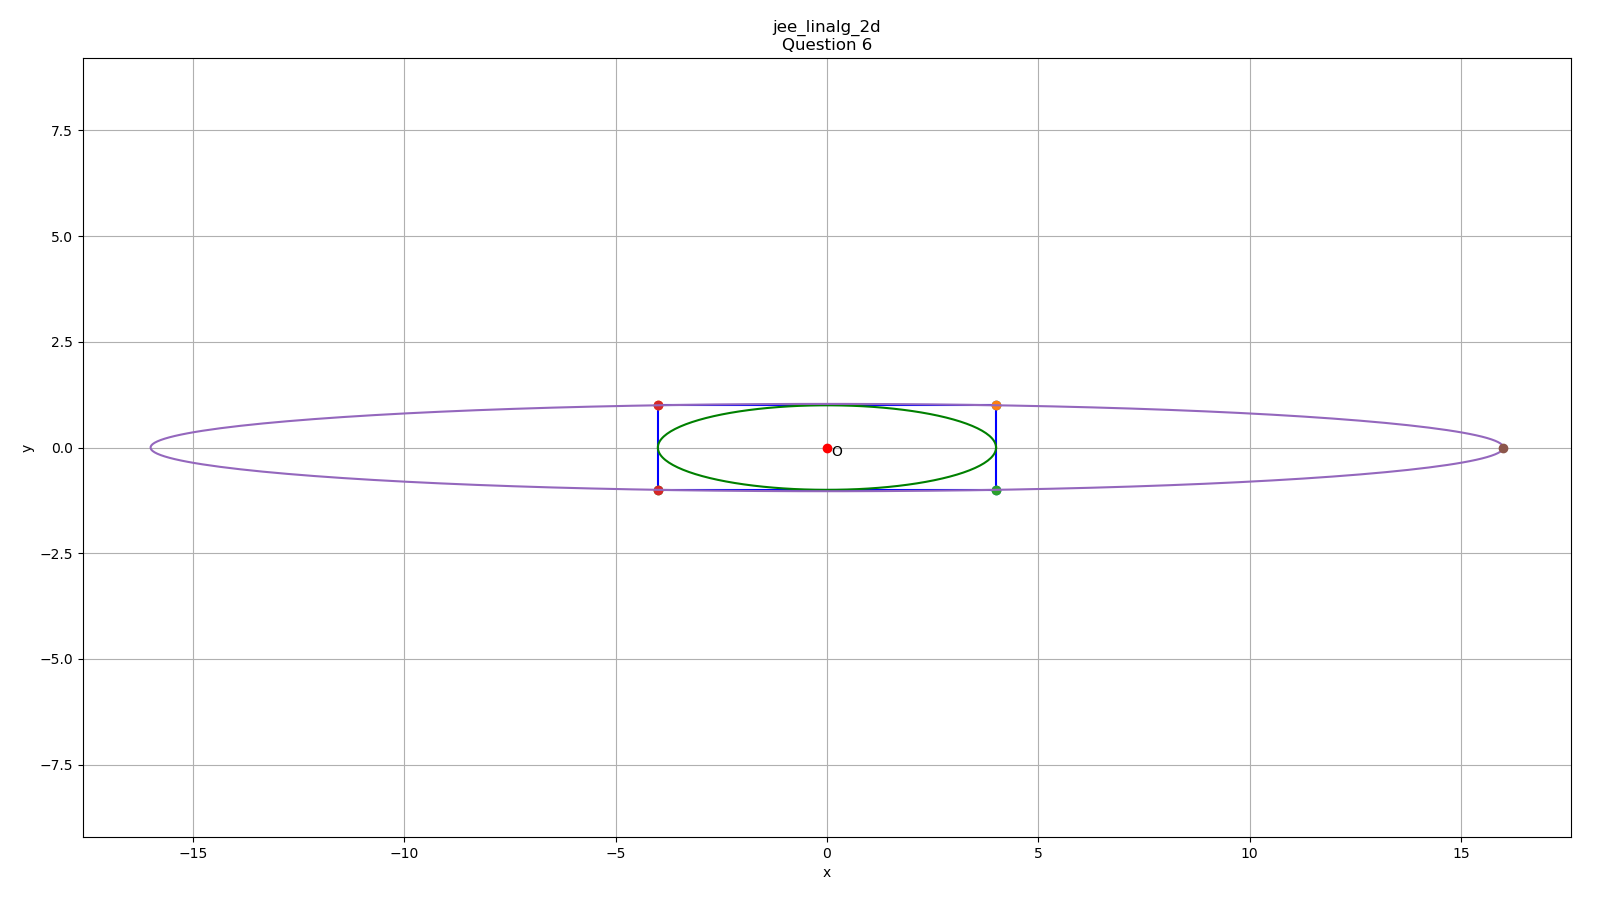
\includegraphics[width=12cm,height=8cm]{./figs/Ellipse2.png}
\end{figure}
\end{frame}
%\begin{frame}
%\frametitle{Introduction}
%\framesubtitle{Literature}
%%\begin{figure}[t!]
%%    \centering
%%    \begin{subfigure}[t]{0.4\columnwidth}
%%        \centering
%%        \includegraphics[width=\columnwidth]{point_source}
%%        \caption{Single point source}
%%\label{fig3:subfig1}        
%%    \end{subfigure}%
%%    ~ 
%%    \begin{subfigure}[t]{0.4\columnwidth}
%%        \centering
%%        \includegraphics[width=\columnwidth]{pointNoPowerDist_new}
%%        \caption{SNR profile}
%%\label{fig3:subfig2}
%%    \end{subfigure}
%%  %  \caption{Average SNR for a BPP. $N=16$}
%%    \label{fig3}
%%  \end{figure}
%
%\end{frame}
%  
%
%
%%

\end{document}
